\chapter{电磁学}

\newpage
{\bf 这里是一段关于电磁学的介绍.}

\newcommand\resistance{
	\begin{tikzpicture}[baseline = {([yshift = -3.5pt] current bounding box.center)}]
		\draw (0, 0) rectangle (0.6, 0.2);
		\draw (-0.3, 0.1) -- (0, 0.1);
		\draw (0.6, 0.1) -- (0.9, 0.1);
	\end{tikzpicture}
}

\newcommand\ammeter{
	
\begin{tikzpicture}[baseline = {([yshift = -3.5pt] current bounding box.center)}]
		\node (A) [circle, draw, scale = 1, inner sep = 1pt, line width = 0.5pt] at (0, 1){\small A};
	\end{tikzpicture}
} % ~{\Large\textcircled{\small A}}~

\newcommand\voltmeter{
	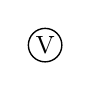
\begin{tikzpicture}[baseline = {([yshift = -3.5pt] current bounding box.center)}]
		\node (V) [circle, draw, scale = 1, inner sep = 1pt, line width = 0.5pt] at (0, 1){\small V};
	\end{tikzpicture}
} % ~{\Large\textcircled{\small V}}~

\newpage
\section{电荷}

\vspace{10pt}
\begin{itemize}
\item 物体能够吸引轻小物体,就说物体带了电,即物体带了\blue{电荷}(electric charge). 带了电荷的物体叫做\blue{带电体}.
\item 使物体带电叫做\blue{起电}. 用摩擦的方式使物体带点叫做\blue{摩擦起电}(electrification by friction).
\item 自然界\blue{只有}两种电荷.
\item 用丝绸摩擦过的玻璃棒带的电荷叫做\blue{正电荷}(positive charge). 用毛皮摩擦过的橡胶棒带的电荷叫做\blue{负电荷}(negative charge).
\item \blue{同种}电荷相互\blue{排斥},\blue{异种}电荷相互\blue{吸引}.
\item 电荷的多少叫做\blue{电荷量}(electric quantity),简称\blue{电量}. 用 \blue{$\bm Q$} 或 \blue{$\bm q$} 表示. 在国际单位制重,电荷量的单位是\blue{库仑}(coulomb),简称\blue{库}. 符号是 \blue{$\bf C$}. 正电荷的电荷量为正值,负电荷的电荷量为负值.
\item \blue{验电器}和\blue{静电计}.
\item 两种电荷互相完全抵消叫做\blue{中和}.
\item 物质是由\blue{分子}构成的,分子是由\blue{原子}构成的.
\item 原子是由带正电的\blue{原子核}和带负电的\blue{电子}(electron)组成的.
\item 原子核是由带正电的\blue{质子}和不带电的\blue{中子}组成的.
\item 每个原子中质子与电子的\blue{数量相等},质子与电子所带的\blue{电荷量相同}.
\item 摩擦起电的本质事电荷从一个物体\blue{转移}到另一个物体.
\item 金属原子中能脱离原子核的束缚而在金属中自由运动的电子叫做\blue{自由电子}(free electron).
\item 失去自由电子的原子叫做\blue{离子}(ion).
\item 质子、电子所带的电荷量(\blue{最小的电荷量})叫做\blue{元电荷}(elementary charge),用 \blue{$\bm e$} 表示. 有:
\mathline{e\approx1.6\times10^{-19}\text{C}}
\item 所有带电体的电荷量都是 $e$ 的整数倍,不是连续变化的,即量子化的.
\item 电子的电荷量 $e$ 与质量 $m_e$ 之比叫做\blue{电子的比荷}(specific charge). 电子的质量 $m_e=9.11\times10^{-31}\text{kg}$,则电子的比荷为:
$$
e:m_e\approx1.76\times10^{11}\text{C}/\text{kg}
$$
\end{itemize}
\newpage
\section{电路}

\subsection{简单电路}
\vspace{10pt}
\begin{itemize}
\item \blue{电路}(electric circuit),即用导线将用电器、电源、开关连接起来.
\item \blue{电源}(power supply),即提供电能的装置,如电池、发电机.
\item \blue{用电器},即消耗电能的装置,如灯泡、电动机.
\item \blue{开关},即控制电路通断的装置,如单刀单掷开关、单刀双掷开关.
\item \blue{导线}通常由绝缘外皮和金属内芯(铜或铝)组成.
\item 处处连通的电路叫做\blue{通路}(\blue{闭合电路}). 某处断开的电路叫做\blue{断路}(\blue{开路}).
\item \blue{直接}用导线将电源的正、负极连接起来的电路叫做\blue{短路}.
\item 闭合电路中,用电器两端被导线直接连通叫做用电器被\blue{短接}.
\item 用符号表示电路连接的图叫做\blue{电路图}.
\item \blue{串联}(series connection)和\blue{并联}(parallel connection).
\item \blue{串联电路}和\blue{并联电路}.
\item 串联电路中各用电器相互影响,并联电路各用电器互不影响.
\end{itemize}